\documentclass[10pt,a4paper]{article}
\usepackage[utf8]{inputenc}
\usepackage[T1]{fontenc}
\usepackage[brazil]{babel}
\usepackage{geometry}
\usepackage{graphicx}
\usepackage{booktabs}
\usepackage{hyperref}
\usepackage{xcolor}
\usepackage{float}
\usepackage{enumitem}
\usepackage{amsmath}
\usepackage{listings}
\usepackage{array}

\geometry{margin=1.5cm}
\setlength{\parskip}{0.24em}
\setlength{\parindent}{0pt}
\setlist{nosep,leftmargin=*}
\hypersetup{colorlinks=true, linkcolor=blue!45!black, urlcolor=blue!45!black, citecolor=blue!45!black, hypertexnames=false}
\lstset{basicstyle=\ttfamily\scriptsize,frame=single,breaklines=true,columns=fullflexible}

\newcommand{\repo}{https://github.com/lcardosott/sus-graph-project}
\newcommand{\repobranch}{gh-pages}
\newcommand{\ghfile}[2]{\href{\repo/blob/\repobranch/#1}{\texttt{#2}}}

\title{\vspace{-1.15cm}Análise de Fluxos e Resiliência do SUS via Teoria dos Grafos}
\author{Lucas Cardoso -- RA 246125 \and Ricardo Andrade Oliveira Bello -- RA 247326}
\date{MC859 -- Entrega Final -- 17 de junho de 2026}

\begin{document}
\maketitle

\textbf{Repositório da implementação:} \url{https://github.com/lcardosott/sus-graph-project}\\
\textbf{Visualização interativa:} \href{https://lcardosott.github.io/sus-graph-project/viz_layer/graph_map_ui.html}{lcardosott.github.io/sus-graph-project/viz\_layer/graph\_map\_ui.html}\\
\textbf{Artefatos principais:}\\
Relatório: \ghfile{report/final_report.tex}{\texttt{report/final\_report.tex}}\\
Visualização: \ghfile{viz_layer/graph_map_ui.html}{\texttt{viz\_layer/graph\_map\_ui.html}}\\
Resultados: \ghfile{algorithm_layer/reports/final_analysis_interpretation.md}{\texttt{algorithm\_layer/reports/}}

\begin{abstract}
Este trabalho modela internações e transferências hospitalares do SUS em 2021 como uma rede direcionada e ponderada. Os vértices representam municípios de residência e hospitais públicos; as arestas representam fluxos observados ou inferidos a partir dos registros do SIH/SUS. A análise combina construção de instâncias, filtros de recorrência e distância, centralidade de intermediação, comunidades Louvain, teste de supressão, k-caminhos e comparação com regiões oficiais de saúde. O principal resultado é que a rede pública hospitalar brasileira aparece conectada quando observada no agregado nacional, mas essa conectividade convive com dependências locais: fluxos recorrentes atravessam regiões oficiais, hospitais especializados atuam como polos estruturais e alguns municípios dependem de poucos destinos externos.
\end{abstract}

\section{Introdução}

O SUS pode ser observado como uma rede: pacientes residem em municípios, são internados em hospitais e, em alguns casos, continuam o atendimento em outro estabelecimento. Essa estrutura não é apenas administrativa; ela revela deslocamentos, polos de atração, redundâncias e gargalos. O objetivo do projeto foi transformar registros públicos de internação em um grafo analisável e usar algoritmos clássicos de grafos para investigar vulnerabilidades de acesso hospitalar.

A pergunta que guiou o trabalho foi: \textit{a rede pública hospitalar observada nos dados é apenas conectada no agregado ou também oferece alternativas locais quando um município depende de poucos hospitais?} Para respondê-la, o projeto partiu do SIH/SUS 2021, integrou referências do CNES e do IBGE, construiu instâncias nacionais e avaliou tanto propriedades globais quanto padrões regionais.

O escopo inicial havia considerado um estudo estadual, mas a implementação final adotou Brasil 2021. A mudança aumentou a escala do grafo, permitiu comparar regiões com realidades distintas e atendeu melhor ao requisito de analisar redes grandes. O recorte final foi restringido a hospitais públicos/SUS, para que os resultados discutissem a rede pública de atendimento e não misturassem fluxos privados ou conveniados fora do escopo principal.

\section{Dados e Pipeline}

Foram usadas três famílias de dados públicos. O SIH/SUS fornece as Autorizações de Internação Hospitalar; o CNES identifica estabelecimentos, natureza pública/SUS e região de saúde; o IBGE fornece códigos territoriais e apoio geográfico \cite{datasus_sih,cnes,ibge_localidades}. A coleta e a preparação foram organizadas de forma modular: os scripts aceitam combinações de ano, meses e UFs, permitindo reproduzir a análise nacional ou gerar recortes menores para validação.

\begin{table}[H]
\centering
\caption{Fontes de dados e artefatos derivados.}
\label{tab:dados}
\scriptsize
\begin{tabular}{p{2.1cm}p{4.0cm}p{7.6cm}}
\toprule
Fonte & Uso no projeto & Campos, referências e artefatos \\
\midrule
SIH/SUS RD 2021 & Internações, origem residencial, perfil clínico e desfecho & \texttt{CODMUNRES}, \texttt{CNES}, \texttt{IDADE}, \texttt{SEXO}, \texttt{RACA\_COR}, \texttt{DIAG\_PRINC}, \texttt{PROC\_REA}, \texttt{DIAS\_PERM}, \texttt{MARCA\_UTI}, \texttt{VAL\_TOT}, óbito e sinais de transferência. \\
CNES & Identificação de hospitais públicos/SUS e regiões de saúde & Catálogo \ghfile{data_layer/reference/catalog/cnes_br_2101_public_hospitals.csv}{cnes\_br\_2101\_public\_hospitals.csv} e campo \texttt{REGSAUDE} da competência 2101. \\
IBGE & Localização territorial & Códigos municipais, UFs e centróides usados quando não havia coordenada mais precisa para o estabelecimento. \\
Artefatos analíticos & Entrada dos algoritmos finais & \ghfile{data_layer/reports/analysis}{data\_layer/reports/analysis}: painéis de hospitais, fluxos de residência, fluxos de transferência, nós e arestas enriquecidos. \\
\bottomrule
\end{tabular}
\end{table}

O pipeline completo começa com a seleção dos arquivos SIH por ano, mês e UF em \ghfile{data_layer/sih_selector.py}{sih\_selector.py}. A execução anual em \ghfile{data_layer/run_sih_year_pipeline.py}{run\_sih\_year\_pipeline.py} projeta colunas relevantes, valida contratos de esquema, cria arestas de residência, infere transferências e gera artefatos intermediários. A etapa final, \ghfile{data_layer/build_public_hospital_analysis.py}{build\_public\_hospital\_analysis.py}, reutiliza os Parquets curados de 2021 e cria as tabelas públicas analisadas pelos algoritmos. Assim, a reprodução da entrega final não exige baixar novamente os dados brutos quando os artefatos curados já existem.

\begin{figure}[H]
\centering
\includegraphics[width=0.48\linewidth]{../viz_layer/reports/graph_sih_br_2021_degree_distribution.png}
\includegraphics[width=0.48\linewidth]{../viz_layer/reports/graph_sih_br_2021_component_size_distribution.png}
\caption{Métricas exploratórias do grafo nacional de 2021: distribuição de graus e distribuição de tamanhos de componentes.}
\label{fig:grafo-base}
\end{figure}

\begin{figure}[H]
\centering
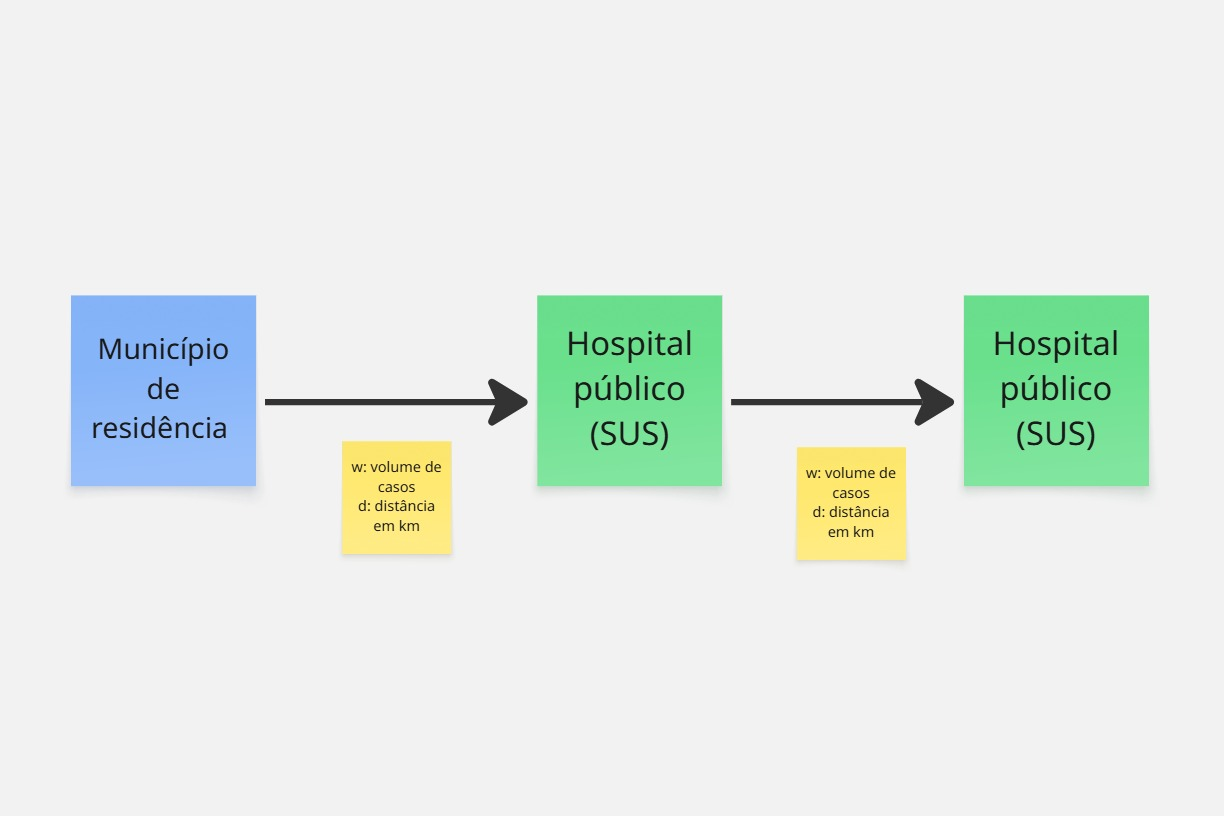
\includegraphics[width=0.72\linewidth]{figures/grafo.jpg}
\caption{Amostra topológica do grafo gerado na etapa de modelagem. A visualização sem mapa evidencia a formação de agrupamentos densos e a presença de ligações entre blocos.}
\label{fig:grafo-topologico}
\end{figure}

O grafo nacional original possui 11.823 nós e 203.184 arestas. No recorte final de hospitais públicos foram encontradas 11.629.005 linhas SIH reconciliadas, 5.875 hospitais públicos presentes no grafo, 188.035 arestas no escopo público, 181.569 fluxos município $\rightarrow$ hospital e 6.466 fluxos hospital $\rightarrow$ hospital. Outros 377 estabelecimentos fora do escopo público foram preservados como controle de qualidade, mas excluídos das conclusões finais.

\section{Construção das Instâncias}

A construção do grafo usou duas instâncias complementares a partir dos mesmos dados: a instância dirigida, que conserva a orientação natural dos fluxos registrados no SIH/SUS, e uma instância projetada não dirigida, derivada dessa base. O grafo dirigido é a representação direta dos eventos: municípios de residência apontam para hospitais de internação e hospitais apontam para hospitais de transferência. Essa versão é essencial para modelar a origem, o destino, o tipo de fluxo e a sequência temporal dos atendimentos.

A instância projetada não dirigida é construída a partir do grafo dirigido, agregando arcos paralelos, somando contagens e mantendo a menor distância entre pares conectados. Esse segundo grafo não busca reconstituir o caminho cronológico exato do paciente, mas sim capturar a conectividade assistencial entre unidades de interesse. Ele é usado para medidas como centralidade de intermediação, comunidades Louvain, teste de supressão dinâmica e análise de redundância de caminhos, porque esses algoritmos exigem uma visão de conjunto baseada em conectividade e caminhos mínimos que não ficam adequadamente definidos num grafo municipalidades $\rightarrow$ hospitais estritamente orientado.

As partes comuns entre as instâncias são claras: ambas compartilham os mesmos nós ativos, as mesmas arestas baseadas nos dados de residência e transferência, as mesmas informações de volume agregado e as mesmas distâncias geográficas. A diferença está na orientação e no propósito analítico. O grafo dirigido preserva a lógica natural dos registros e serve para montar o escopo, enquanto a projeção não dirigida preserva a estrutura topológica relevante para mapear referências, comunidades funcionais e alternativas de rota.

O conjunto de vértices $V$ contém dois tipos de vértices: municípios de residência e hospitais públicos. No grafo dirigido, uma aresta de residência $u \rightarrow v$ liga o município de residência do paciente ao hospital de internação; uma aresta de transferência $h_i \rightarrow h_j$ liga dois hospitais quando os registros indicam continuidade provável de atendimento. O peso $w(e)$ representa volume agregado e $d(e)$ representa distância geográfica aproximada.

As transferências exigiram maior cuidado porque a base não oferece, de forma limpa e universal, uma lista explícita de origem e destino. A implementação adotou uma heurística conservadora de quatro pilares em \ghfile{data_layer/transfer_matching.py}{transfer\_matching.py}: sinal de transferência por campo ou motivo de saída validado, janela temporal de 24 a 48 horas entre alta e nova internação, continuidade demográfica por sexo e idade, e continuidade clínica por capítulo CID-10. O CID-10 é a Classificação Internacional de Doenças, usada nos registros hospitalares para codificar diagnósticos; neste trabalho, ele foi usado de forma agregada para verificar se a internação seguinte parecia pertencer ao mesmo quadro clínico. Quando havia múltiplos candidatos, a escolha priorizava menor intervalo temporal, CID exato e identificador de destino estável. Esse procedimento não deve ser lido como rastreamento individual perfeito, mas como uma forma reprodutível de inferir relações estruturais recorrentes entre hospitais.

A distância entre os pontos foi calculada pela fórmula de Haversine:
\begin{equation}
 d = 2r \arcsin \sqrt{
 \sin^2\left(\frac{\Delta \phi}{2}\right) +
 \cos(\phi_1)\cos(\phi_2)\sin^2\left(\frac{\Delta \lambda}{2}\right)
 },
\label{eq:haversine}
\end{equation}
em que $\phi$ é latitude, $\lambda$ é longitude e $r$ é o raio aproximado da Terra. Quando a coordenada exata do hospital não estava disponível, foi usado o centróide do município. Essa decisão aumenta a cobertura nacional, mas limita interpretações finas dentro de cidades grandes.

Para reduzir ruído, as instâncias algorítmicas usaram dois filtros. O primeiro é de recorrência: fluxos residência $\rightarrow$ hospital entram com pelo menos 5 ocorrências e transferências hospital $\rightarrow$ hospital com pelo menos 2 ocorrências. O segundo é de distância mínima: foram geradas instâncias de 25 km e 50 km. O corte de 25 km captura fricções regionais e locais que já podem ser relevantes para pacientes; o corte de 50 km é mais seletivo e destaca dependências mais longas. Esses cortes não são percentuais da base: são limiares geográficos aplicados às arestas depois da agregação.

\begin{lstlisting}[caption={Construção da instância analítica filtrada.}]
para cada aresta e do grafo publico:
  se e.tipo = residencia e e.volume < 5: descartar
  se e.tipo = transferencia e e.volume < 2: descartar
  se e.distancia_km < distancia_minima: descartar
  manter e na instancia

G_dir = grafo dirigido com as arestas mantidas
G_proj = projecao nao dirigida ponderada por volume e distancia
usar maior componente de G_proj para centralidade, comunidades e stress test
\end{lstlisting}

\section{Implementação}

A implementação foi dividida em camadas para manter rastreabilidade e facilitar reexecuções parciais. A \texttt{data\_layer} concentra coleta, validação e tabelas analíticas; a \texttt{model\_layer} constrói o grafo anual em GEXF; a \texttt{filter\_engine} implementa filtros reutilizáveis de distância, tipo e recorrência; a \texttt{algorithm\_layer} executa os métodos finais; a \texttt{viz\_layer} produz mapas, figuras e uma visualização interativa leve.

Os algoritmos finais estão em \ghfile{algorithm_layer/public_hospital_analysis.py}{public\_hospital\_analysis.py} e \ghfile{algorithm_layer/regional_flow_analysis.py}{regional\_flow\_analysis.py}. No código principal de análise, o pipeline começa em \texttt{parse\_args()}, que define parâmetros reproduzíveis como limiares de residência, transferência, distância e amostragem para centralidade. A função \texttt{load\_inputs()} lê os artefatos curados de nó e aresta, normaliza contagens e converte distâncias para valores numéricos.

A função \texttt{filter\_edges()} aplica os filtros principais usados no relatório: conserva arestas de residência com pelo menos 5 ocorrências, arestas de transferência com pelo menos 2 ocorrências e arestas com distância acima do limiar escolhido. Em seguida, \texttt{build\_directed\_graph()} constrói o grafo direcionado com atributos como \texttt{edge\_type}, \texttt{transfer\_count} e \texttt{distance\_km}, além de manter os metadados de cada nó. A partir desse grafo registra\-do, \texttt{weighted\_projection()} gera a projeção não dirigida ponderada por volume, somando \texttt{transfer\_count} para arestas repetidas e preservando a menor distância entre pares quando existem múltiplas arestas paralelas.

A maior componente da projeção é selecionada por \texttt{largest\_component()}, e, nessa instância, são executadas as análises de conectividade. \texttt{community\_reports()} usa \texttt{nx.community.louvain\_communities()} com peso \texttt{transfer\_count} para identificar comunidades funcionais. \texttt{top\_facility\_centrality()} calcula a centralidade de intermediação aproximada com amostragem (	exttt{k} padrão 200), filtrando apenas hospitais na saída. \texttt{dynamic\_stress()} executa o teste de supressão dinâmica: amostra até 120 nós, remove iterativamente o hospital de maior centralidade e registra a evolução do tamanho da maior componente e do caminho médio.

A camada de regionalização em \texttt{regional\_flow\_analysis.py} junta os dados de arestas com o catálogo de municípios e regiões de saúde. Ela calcula um campo \texttt{same\_health\_region} e classifica fluxos como intra-região, inter-região ou desconhecidos. Os relatórios de saída agrupam resultados para bandas de 25 km e 50 km, permitem comparar residência e transferência, e destacam municípios com dependência externa total em relação aos fluxos recorrentes.

Essa distinção é a base técnica para explicar por que a direção é mantida na modelagem e por que a projeção não dirigida é usada nas análises de conectividade. Em um grafo estritamente dirigido, muitos caminhos município $\rightarrow$ hospital não retornam e as medidas ficariam dominadas pela orientação administrativa das arestas. A projeção ponderada preserva a informação de volume e de distância, tornando possível analisar a estrutura de referência e a redundância de rotas sem perder a origem do fluxo.

\begin{table}[H]
\centering
\caption{Arquivos de implementação e saídas principais dos algoritmos.}
\label{tab:arquivos-algoritmos}
\scriptsize
\begin{tabular}{p{0.18\linewidth}p{0.29\linewidth}p{0.45\linewidth}}
\toprule
Método & Implementação & Saídas principais \\
\midrule
Centralidade de intermediação &
\ghfile{algorithm_layer/public_hospital_analysis.py}{public\_hospital\_analysis.py} &
\ghfile{algorithm_layer/reports/final_2021_public_hospitals_50km_centrality.csv}{centrality.csv} e
\ghfile{algorithm_layer/reports/final_2021_public_hospitals_50km_summary.json}{summary.json}. \\
Comunidades Louvain &
\ghfile{algorithm_layer/public_hospital_analysis.py}{public\_hospital\_analysis.py} &
\ghfile{algorithm_layer/reports/final_2021_public_hospitals_50km_communities.csv}{communities.csv} e
\ghfile{algorithm_layer/reports/final_2021_public_hospitals_50km_community_region_overlap.csv}{community\_region\_overlap.csv}. \\
Supressão dinâmica &
\ghfile{algorithm_layer/public_hospital_analysis.py}{public\_hospital\_analysis.py} &
\ghfile{algorithm_layer/reports/final_2021_public_hospitals_50km_stress_dynamic.csv}{stress\_dynamic.csv} e
\ghfile{algorithm_layer/reports/final_2021_public_hospitals_50km_sensitivity_matrix.csv}{sensitivity\_matrix.csv}. \\
K-caminhos mais curtos &
\ghfile{algorithm_layer/public_hospital_analysis.py}{public\_hospital\_analysis.py} &
\ghfile{algorithm_layer/reports/final_2021_public_hospitals_50km_k_path_redundancy.csv}{k\_path\_redundancy.csv}. \\
Fluxo máximo/corte mínimo &
\ghfile{algorithm_layer/public_hospital_analysis.py}{public\_hospital\_analysis.py} &
\ghfile{algorithm_layer/reports/final_2021_public_hospitals_50km_min_cut_capacity.csv}{min\_cut\_capacity.csv} e
\ghfile{algorithm_layer/reports/final_2021_public_hospitals_50km_min_cut_facilities.csv}{min\_cut\_facilities.csv}. \\
Regiões de saúde &
\ghfile{algorithm_layer/regional_flow_analysis.py}{regional\_flow\_analysis.py} &
\ghfile{algorithm_layer/reports/regional_2021_public_hospitals_overall.csv}{regional\_overall.csv},
\ghfile{algorithm_layer/reports/regional_2021_public_hospitals_regional_mismatch.csv}{regional\_mismatch.csv} e
\ghfile{algorithm_layer/reports/regional_2021_public_hospitals_municipality_dependency.csv}{municipality\_dependency.csv}. \\
\bottomrule
\end{tabular}
\end{table}

A validação combinou testes automatizados e reconciliação de totais. Os testes cobrem seleção SIH, contratos de esquema, enriquecimento de nós, filtros, construção do recorte público e algoritmos. Além disso, os totais do grafo, das tabelas públicas e dos relatórios finais foram comparados por arquivos de resumo JSON. Essa estratégia não elimina limitações dos dados públicos, mas torna as transformações auditáveis.

\section{Algoritmos e Resultados}

\subsection{Centralidade de Intermediação}

A centralidade de intermediação (\textit{betweenness centrality}) mede quanto um vértice aparece em caminhos mínimos entre outros pares de vértices. No contexto do projeto, um hospital com alta intermediação não é apenas um hospital com grande volume; ele atua como ponte entre municípios, regiões e corredores de atendimento. A distância foi usada como custo dos caminhos, e a métrica foi aproximada por amostragem para viabilizar a execução em máquina local.

\begin{lstlisting}[caption={Centralidade de intermediação em hospitais públicos.}]
G = maior componente da projecao ponderada
calcular betweenness em G usando distancia_km como custo
selecionar apenas vertices do tipo hospital
ordenar hospitais por betweenness decrescente
\end{lstlisting}

\begin{figure}[H]
\centering
\includegraphics[width=0.73\linewidth]{figures/map_central_hospitals.png}
\caption{Distribuição espacial dos hospitais de maior intermediação no corte de 50 km, sobreposta a uma amostra dos corredores filtrados.}
\label{fig:mapa-centralidade}
\end{figure}

\begin{figure}[H]
\centering
\includegraphics[width=0.73\linewidth]{../viz_layer/reports/top_central_facilities_public_hospitals.png}
\caption{Hospitais públicos com maior centralidade de intermediação nas instâncias finais.}
\label{fig:centralidade}
\end{figure}

No corte de 50 km, os principais hospitais por centralidade foram Fundação Pio XII Barretos, Hospital Amaral Carvalho Jaú, Hospital São Vicente de Paulo, Hospital Regional Tibério Nunes, Hospital Municipal Esaú Matos, Hospital das Clínicas FAEPA Ribeirão Preto e Hospital de Base de São José do Rio Preto. Esses hospitais aparecem no topo da métrica porque conectam muitos municípios e outros hospitais por caminhos de menor custo geográfico dentro da projeção.

Um hospital com alta centralidade funciona como um eixo na rede assistencial. Socialmente, isso significa que ele concentra muito mais do que internações: concentra decisões de encaminhamento, transporte de pacientes, acompanhamento de casos complexos e eventual sobrecarga de sistemas de regulação. Existe um problema por trás disso. Alta centralidade pode ser sintoma de desigualdade de oferta local e de dependência de poucos polos. Quando o atendimento de um município ou de uma região depende fortemente de um único hospital central, a falha desse hospital — por falta de leitos, greves, crises sanitárias ou restrição de capacidade — impacta um conjunto extenso de municípios.

As implicações práticas e sociais são múltiplas. Primeiro, o planejamento de capacidade deve reconhecer que esses hospitais não são apenas grandes em volume, mas são críticos para a conectividade da rede. Segundo, políticas de regionalização precisam considerar os fluxos reais e não apenas a localização de leitos oficiais; um hospital de alta centralidade pode exigir apoio extra em transporte, regulação e infraestrutura de acolhimento de familiares. Terceiro, o fato de alguns hospitais assumirem esse papel de ponte reforça a necessidade de fortalecer alternativas locais, distribuindo recursos e especialidades de forma a reduzir a dependência de trajetos longos e policentrar o atendimento público.

\subsection{Comunidades Louvain}

O método Louvain agrupa vértices que têm conexões internas mais fortes do que conexões com o restante da rede. A métrica otimizada é a modularidade; no projeto, o peso das arestas foi o volume agregado. As comunidades não foram tratadas como regiões oficiais, mas como regiões funcionais sugeridas pelos próprios fluxos.

\begin{figure}[H]
\centering
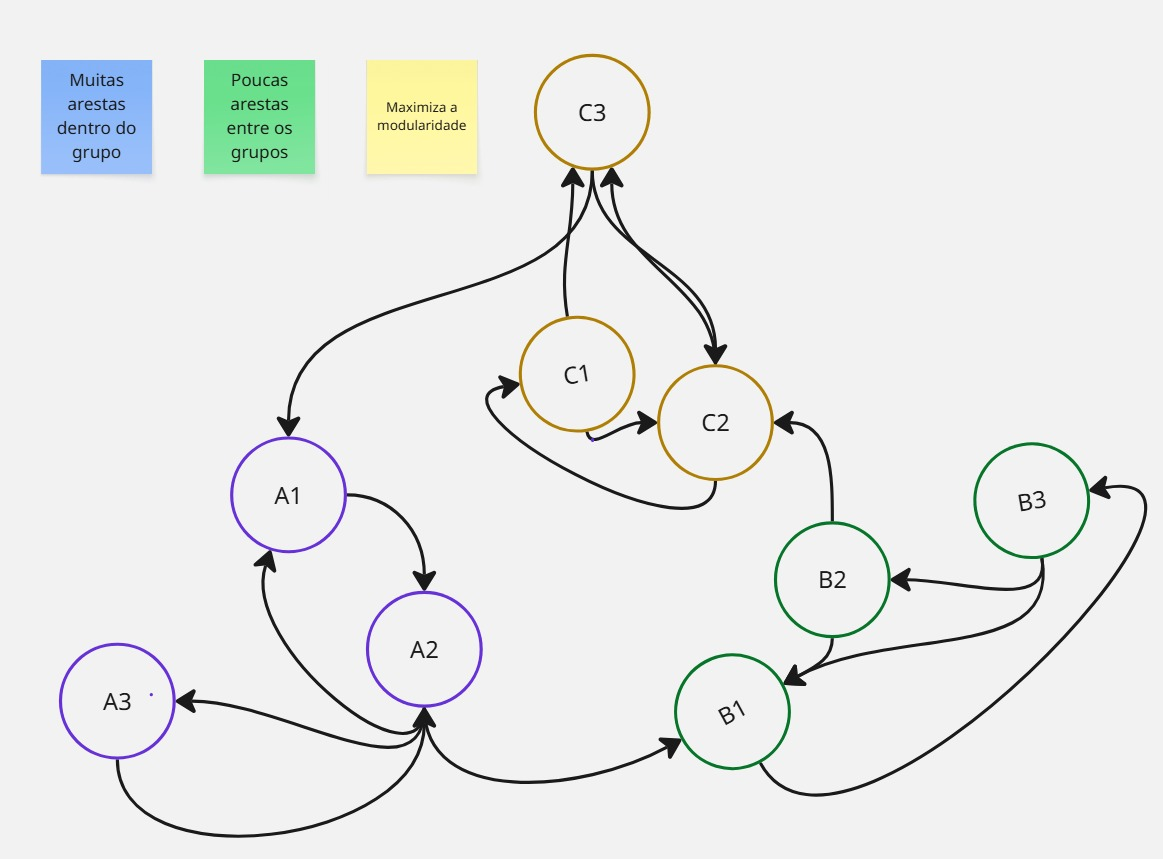
\includegraphics[width=0.68\linewidth]{figures/louvain.jpg}
\caption{Intuição do Louvain: comunidades concentram muitas arestas internas e poucas arestas entre grupos, maximizando modularidade.}
\label{fig:louvain}
\end{figure}

As instâncias principais tiveram 49 comunidades no corte de 25 km e 43 comunidades no corte de 50 km. A redução ocorre porque o corte de 50 km remove parte dos deslocamentos regionais curtos e deixa uma rede mais seletiva, concentrada em corredores longos. Essa diferença mostra que a lógica de comunidade muda quando se faz um filtro mais rígido: a rede funcional se torna menos fragmentada e mais dominada por grandes blocos de fluxo de alta distância.

Uma comunidade Louvain no contexto dos hospitais representa um conjunto de municípios e hospitais que compartilham rotas recorrentes e que, portanto, funcionam como uma unidade assistencial de fato. O problema social surge quando essas comunidades não coincidem com as regiões oficiais de saúde. Nesse caso, as decisões de gestão, financiamento e regulação podem estar desalinhadas com os fluxos reais de pacientes e as necessidades efetivas das populações.

Na prática, pertencer a uma mesma comunidade Louvain significa que municípios e hospitais estão integrados por atendimentos frequentes. Isso pode ser positivo, pois sugere coesão funcional, mas também revela vulnerabilidades: uma comunidade muito concentrada em poucos hospitais ou em uma mesma direção pode sofrer com restrição de alternativas se um destino preferencial estiver sobrecarregado. A implicação social é que políticas de reorganização precisam reconhecer esses mosaicos funcionais e apoiar a coordenação entre regiões, especialmente quando as comunidades atravessam estados ou códigos de região de saúde.

\subsection{Supressão Dinâmica}

O teste de supressão remove iterativamente hospitais com maior intermediação e recalcula a maior componente e o caminho médio amostrado. A pergunta não é se a rede "deixa de existir", mas se a retirada de polos centrais alonga caminhos ou fragmenta a conectividade.

\begin{figure}[H]
\centering
\includegraphics[width=0.68\linewidth]{figures/stress_test_algorithm.png}
\caption{Procedimento do teste de supressão dinâmica: recalcular intermediação, remover um polo e medir o efeito sobre conectividade e rotas.}
\label{fig:stress-algoritmo}
\end{figure}

\begin{lstlisting}[caption={Teste de supressão dinâmica.}]
G = maior componente da instancia filtrada
registrar tamanho da componente e caminho medio amostrado
para passo em 1..5:
  recalcular betweenness dos hospitais em G
  remover hospital com maior betweenness
  recalcular maior componente e caminho medio amostrado
\end{lstlisting}

\begin{figure}[H]
\centering
\includegraphics[width=0.49\linewidth]{../viz_layer/reports/resilience_largest_component_public_hospitals.png}
\includegraphics[width=0.49\linewidth]{../viz_layer/reports/resilience_stress_path_increase_public_hospitals.png}
\caption{Efeito da supressão de hospitais centrais sobre maior componente e caminho médio amostrado.}
\label{fig:stress}
\end{figure}

\begin{table}[H]
\centering
\caption{Resumo das instâncias e do stress test após cinco remoções.}
\label{tab:instancias}
\begin{tabular}{lrrrrr}
\toprule
Instância & Nós & Arestas & Comunidades & Maior comp. final & Aumento caminho \\
\midrule
25 km & 8.622 & 61.706 & 49 & 99,9072\% & 0,7839\% \\
50 km & 7.750 & 47.739 & 43 & 99,4702\% & 1,2597\% \\
\bottomrule
\end{tabular}
\end{table}

O resultado agregado indica que a rede nacional não se fragmenta facilmente. Porém, essa conclusão precisa ser lida com cuidado: conectividade nacional não mede disponibilidade de vaga, tempo real de deslocamento ou impacto local. A rede pode preservar 99\% da maior componente enquanto um município específico perde seu destino de referência. Por isso, o stress test é mais útil como contraste: ele mostra robustez global, e essa robustez torna ainda mais necessário olhar dependências municipais.

\subsection{K-Caminhos Mais Curtos}

Os k-caminhos mais curtos (\textit{k-shortest paths}) foram usados para avaliar redundância. Em vez de perguntar apenas qual é o menor caminho entre uma origem e um hospital, o método pergunta quais seriam as próximas melhores alternativas. Assim, para um par município $\rightarrow$ hospital de alto volume, calculamos o melhor caminho $k_1$ e, quando existente, um segundo caminho $k_2$ que não repete exatamente a mesma rota. A razão $d(k_2)/d(k_1)$ indica o custo relativo da alternativa.

Essa leitura é importante porque conectividade não significa substituição fácil. Se $k_2$ tem distância parecida com $k_1$, há alguma redundância prática. Se $k_2$ é duas, três ou cinco vezes mais longo, a rede até possui uma alternativa topológica, mas ela pode ser ruim como opção assistencial. Quando apenas um caminho foi encontrado na instância filtrada, o par foi marcado como sem alternativa relevante dentro dos critérios de recorrência e distância adotados.

No corte de 50 km, entre os pares analisados, houve casos com três caminhos encontrados, mas com segunda alternativa acima de duas vezes a distância do melhor caminho. Também houve pares com apenas um caminho relevante dentro da instância filtrada. Isso mostra que redundância não é binária: uma região pode estar conectada no grafo e ainda assim depender de alternativas longas ou frágeis.

\begin{figure}[H]
\centering
\includegraphics[width=0.74\linewidth]{figures/k_path_redundancy.png}
\caption{Razão entre o segundo e o primeiro caminho mais curto em pares de alto volume no corte de 50 km. Valores acima de 2 indicam alternativas formalmente existentes, mas possivelmente pouco substitutivas.}
\label{fig:k-caminhos}
\end{figure}

\subsection{Fluxo Máximo e Corte Mínimo}

O projeto incluiu uma aproximação de fluxo máximo/corte mínimo, mas ela foi rebaixada para resultado exploratório. O teorema max-flow/min-cut é adequado para estudar gargalos quando há capacidades confiáveis nas arestas e nos destinos. Neste trabalho, a capacidade disponível foi aproximada pelo volume anual observado, que não equivale a leitos operacionais, equipe, ocupação simultânea, especialidade ou disponibilidade temporal. Assim, a implementação fica no repositório como base para continuidade, mas as conclusões finais não dependem dela.

Mesmo assim, a análise exploratória traz uma descoberta social relevante: a rede não é apenas conectada, ela é funcionalmente desigual. Existem corredores assistenciais e nós que carregam mais fluxo quando medimos capacidade implícita. Em termos sociais, isso significa que alguns hospitais e rotas de transferência são estruturas de referência para várias municipalidades e que sua limitação tem impacto direto em pacientes, famílias e sistemas de regulação.

A implicação prática é clara: políticas de acesso devem olhar além da quantidade total de leitos e considerar a forma como os fluxos reais circulam. A análise sugere que o SUS público brasileiro em 2021 apresenta tanto conectividade global quanto pontos de fragilidade local, e que a simples existência de uma rota de transferência não garante que essa rota seja uma alternativa assistencial razoável.

\section{Regiões Oficiais e Dependência Municipal}

O objetivo desta análise de regionalização foi confrontar o acesso efetivo observado nos dados com o desenho oficial de regiões de saúde do CNES. Queríamos verificar até que ponto os fluxos recorrentes de residência $\rightarrow$ hospital e de transferência hospitalar respeitam os limites das regiões oficiais, e identificar onde a prática efetiva rompe a estrutura administrativa.

Existem problemas por trás dessa comparação. Um fluxo recorrente que cruza região oficial de saúde pode indicar que a oferta dentro da região é insuficiente, que há falta de especialidade local ou que a regulação regional não consegue atender a demanda. Também pode revelar custos sociais adicionais para pacientes e famílias: deslocamentos mais longos, maior tempo de espera, necessidade de hospedagem e perda de tempo produtivo. Quando esses fluxos se concentram em poucos destinos externos, a vulnerabilidade se intensifica.

As implicações práticas e sociais são importantes. Se a rede real não coincide com as regiões oficiais, as decisões de alocação de recursos e a governança regional precisam ser adaptadas. Além de apontar possíveis gaps de capacidade, essa análise sugere a necessidade de maior coordenação interestadual e inter-regional, políticas de transporte sanitário e revisão de fluxos de referência que considerem as rotas efetivas dos pacientes.

\begin{table}[H]
\centering
\caption{Fluxos recorrentes que cruzam região oficial de saúde.}
\label{tab:regioes}
\scriptsize
\begin{tabular}{llrrrrr}
\toprule
Distância & Tipo & Arestas & Fluxo total & Fora da região & Parcela fora & Dist. média pond. \\
\midrule
25 km & Residência & 60.646 & 3.488.440 & 1.117.796 & 32,04\% & 86,96 km \\
25 km & Transferência & 1.060 & 3.585 & 1.868 & 52,11\% & 148,14 km \\
50 km & Residência & 46.938 & 1.942.302 & 850.778 & 43,80\% & 128,20 km \\
50 km & Transferência & 801 & 2.748 & 1.676 & 60,99\% & 182,08 km \\
\bottomrule
\end{tabular}
\end{table}

A Tabela \ref{tab:regioes} concentra um dos achados centrais. Aqui, "fora da região" não significa necessariamente sair do estado. A comparação usa a região oficial de saúde do CNES, identificada pelo campo \texttt{REGSAUDE}; um mesmo estado possui várias regiões de saúde, por isso muitos cruzamentos aparecem como PE-0004 $\rightarrow$ PE-0001, SP-0201 $\rightarrow$ SP-0101 ou BA-0003 $\rightarrow$ BA-0001. Esses são fluxos entre regiões administrativas diferentes dentro da mesma UF. Cruzamentos de estado também existem e foram calculados separadamente como \textit{cross UF}, mas não são o foco desta tabela.

Quando os fluxos são recorrentes, parte expressiva do atendimento ultrapassa a região oficial de saúde. Isso não significa que todo deslocamento inter-regional seja problemático: alta complexidade frequentemente exige referência externa. O sinal de vulnerabilidade aparece quando o deslocamento é repetido, longo e concentrado em poucos destinos.

O perfil geográfico desses casos reforça um ponto relevante: as regiões mais dependentes tendem a ser municípios do interior e áreas periféricas, não necessariamente polos litorâneos. Entre os 527 municípios com 100\% do fluxo recorrente direcionado a um único destino externo, há muitos exemplos do interior de Minas Gerais, São Paulo, Mato Grosso, Pará e Rio Grande do Sul, bem como municípios amazônicos e nordestinos que percorrem distâncias superiores a 1.000 km para acessar hospitais especializados.

Esses padrões aparecem também nos principais corredores de mismatch. Os fluxos de maior volume incluem deslocamentos interior\textnormal{--}capital e interior\textnormal{--}polo regional, como Pernambuco para Recife, Goiás para Brasília, Ceará para Fortaleza, Bahia para Salvador, Pará para Belém, Rio Grande do Sul para Porto Alegre e região de Ribeirão Preto para a capital paulista. Esses exemplos são consistentes com uma dependência de oferta em regiões menos servidas e com uma desigualdade de acesso que atravessa fronteiras administrativas.

\begin{figure}[H]
\centering
\includegraphics[width=0.72\linewidth]{figures/regional_cross_share.png}
\caption{Parcela do fluxo recorrente que cruza regiões oficiais de saúde, por tipo de aresta e limiar de distância.}
\label{fig:fluxos-fora-regiao}
\end{figure}

\begin{figure}[H]
\centering
\includegraphics[width=0.72\linewidth]{figures/regional_mismatch_top.png}
\caption{Principais corredores região $\rightarrow$ região no corte de 50 km. A anotação ao lado das barras indica também a participação do corredor no fluxo de origem.}
\label{fig:corredores-regionais}
\end{figure}

\begin{table}[H]
\centering
\caption{Exemplos de dependência municipal no corte de 50 km.}
\label{tab:dependencia}
\scriptsize
\begin{tabular}{p{3.2cm}p{5.0cm}rrr}
\toprule
Município & Principal destino externo & Fluxo & Participação & Distância \\
\midrule
Serra Nova Dourada -- MT & Hospital Regional de Água Boa & 96 & 100\% & 241,2 km \\
Caiana -- MG & Hospital do Câncer de Muriaé & 70 & 100\% & 65,4 km \\
Dom Cavati -- MG & Hospital Municipal Eliane Martins & 58 & 100\% & 50,1 km \\
Bujaru -- PA & Hospital Regional Público Dr. Abelardo Santos & 47 & 100\% & 56,1 km \\
Santana do Cariri -- CE & Hospital Maternidade São Vicente de Paulo & 41 & 100\% & 50,8 km \\
\bottomrule
\end{tabular}
\end{table}

Esses exemplos mostram por que a média nacional é insuficiente. Para a rede inteira, uma remoção pode alterar pouco a maior componente; para um município que concentra 100\% do fluxo filtrado em um destino fora de sua região, a perda desse destino representa uma fragilidade concreta. Em um estudo mais focalizado, uma extensão natural seria escolher um estado ou macrorregião, validar a regionalização com bases locais e analisar impactos percentuais por município e especialidade.

\section{Visualização}

A visualização final foi desenhada como camada de apresentação analítica, não como tentativa de renderizar todas as 188 mil arestas no navegador. O script \ghfile{viz_layer/build_final_map_layers.py}{build\_final\_map\_layers.py} gera o arquivo leve \ghfile{viz_layer/reports/final_map_layers.json}{final\_map\_layers.json}, com corredores principais, hospitais centrais, nós removidos no stress test, comunidades e exemplos de dependência municipal.

No \ghfile{viz_layer/graph_map_ui.html}{graph\_map\_ui.html}, o usuário pode alternar presets de 25 km, 50 km, hospitais centrais, stress test e dependência municipal. A interface evita desenhar tudo ao mesmo tempo: trabalha com camadas reduzidas, oculta arestas durante navegação e redesenha em blocos. Essa decisão foi necessária porque a visualização bruta ficava pesada, enquanto a versão guiada preserva a mensagem analítica e roda em computadores comuns. Como alternativa estática, \ghfile{viz_layer/reports/final_showcase.html}{final\_showcase.html} reúne gráficos e tabelas principais.

\begin{figure}[H]
\centering
\includegraphics[width=0.49\linewidth]{figures/map_25km.png}
\includegraphics[width=0.49\linewidth]{figures/map_50km.png}
\caption{Amostras estáticas dos presets de 25 km e 50 km da camada final: o corte de 25 km preserva mais fricções regionais, enquanto 50 km destaca corredores longos e seletivos.}
\label{fig:presets-mapa}
\end{figure}

\begin{figure}[H]
\centering
\includegraphics[width=0.64\linewidth]{figures/map_dependency_examples.png}
\caption{Exemplos geográficos de dependência municipal usados pela camada de visualização final.}
\label{fig:mapa-dependencias}
\end{figure}

\section{Limitações e Interpretação}

Os resultados devem ser interpretados como análise de acesso realizado, não de necessidade total. O SIH mostra internações que ocorreram; ele não mostra pacientes que não conseguiram vaga, demanda reprimida ou tempo de espera. Além disso, a base anual não mede capacidade simultânea: volume em 2021 não informa quantos leitos estavam disponíveis em uma semana crítica, quais equipes estavam ativas ou quais especialidades eram necessárias.

Outra limitação é espacial. A distância Haversine aproxima deslocamento em linha geodésica, mas não mede tempo por estrada, transporte público, rios ou barreiras locais. Em áreas rurais e amazônicas, 50 km podem representar realidades muito diferentes. A inferência de transferências também é probabilística e conservadora; ela é útil para padrões estruturais, mas não substitui uma base clínica de regulação com identificadores explícitos de origem e destino.

Por fim, a análise regional depende do \texttt{REGSAUDE} disponível no CNES/ST. Como foram encontrados conflitos e ausências, a comparação com regiões oficiais é uma aproximação. Ainda assim, o volume de fluxos fora da região é suficientemente alto para indicar uma tensão real entre o desenho administrativo e os caminhos observados nos dados.

\section{Analise dos resultados}

Este projeto mostrou que a análise de fluxos hospitalares do SUS em 2021 ganha profundidade quando combinada com grafos e filtros pensados para a prática assistencial. O grafo dirigido permitiu modelar residências, internações e transferências de forma fiel ao SIH/SUS, enquanto a projeção não dirigida manteve a estrutura de referência necessária para medir conectividade, centralidade e redundância.

Os resultados obtidos apontam para um conjunto de problemáticas relevantes. A centralidade de intermediação revelou hospitais que funcionam como polos estruturais de uma rede nacional: eles são mais do que grandes fornecedores de vagas, são pontos de passagem que conectam municípios e regiões. Essa posição aumenta a vulnerabilidade da rede, porque uma falha nesses nós afeta fluxos que atravessam estados e macrorregiões. Em paralelo, as comunidades Louvain ilustraram que a rede funcional nem sempre coincide com as regiões oficiais de saúde, mostrando blocos de fluxo que podem atravessar divisões administrativas e demandar maior coordenação entre regiões.

O achado sobre regionalização confirma outra tensão: cerca de 44\% dos fluxos de residência recorrentes e 61\% dos fluxos de transferência recorrentes no corte de 50 km ocorrem fora da região oficial de saúde. Esses números não apenas evidenciam um desalinhamento entre desenho administrativo e prática assistencial, mas também sugerem custos sociais e de gestão adicionais para pacientes, famílias e reguladores. Há municípios que dependem de 100\% de um único destino externo em fluxos recorrentes, o que traduz fragilidade local mesmo em uma rede nacional estatisticamente robusta.

Em outras palavras, a rede pública hospitalar brasileira de 2021 é conectada no agregado, mas apresenta padrões de dependência e desigualdade regionais. A robustez do maior componente coexistiu com dependências municipais pontuais e com blocos funcionais que não cabem perfeitamente no mapa oficial. As regiões mais dependentes tendem a ser municípios do interior e áreas periféricas, incluindo localidades do Norte, Nordeste e Centro-Oeste que viajam longas distâncias para hospitais de referência. Essa dicotomia é central para entender o valor do trabalho: ele não mede apenas conectividade, mas também expõe onde essa conectividade pode ser frágil, concentrada ou desalinhada.

\section{Conclusão}

A análise mostra que o SUS público de 2021 é simultaneamente conectado e desigual: a malha hospitalar nacional sustenta uma grande componente interligada, mas fluxos recorrentes e dependências únicas expõem fragilidades regionais. Hospitais de alta intermediação e comunidades funcionais desalinhadas com regiões oficiais de saúde apontam para uma governança que precisa considerar os fluxos reais, não apenas a infraestrutura declarada.

Os cortes geográficos de 25 km e 50 km permitiram enxergar duas faces do fenômeno. No nível mais local, há fricções e dependências de poucos destinos; no nível mais amplo, há corredores que atravessam regiões e estados. Esses dois veios juntos sugerem que a política pública deve atuar tanto na descentralização de alternativas quanto na articulação de estruturas de referência mais robustas.

Por fim, o trabalho reafirma que emoção social e algoritmo não são opostos: uma abordagem de grafos aplicada a dados públicos pode transformar observações de fluxo em informações acionáveis. O principal ganho é esse: tornar visível onde o SUS funciona como rede conectada e onde ele ainda precisa de ajustes para reduzir dependência, desigualdade e vulnerabilidade.

\section{Referências}

\nocite{*}
\bibliographystyle{plain}
\bibliography{references}
\end{document}
